\documentclass[12pt,a4paper]{article}

% Necessary Packages Only
\usepackage{amsmath}
\usepackage{amssymb}
\usepackage{geometry}
\usepackage{graphicx}
\usepackage{textcomp}

\newcommand{\rupee}{\textrm{Rs.}}

\geometry{top=2.5cm, bottom=2.5cm, left=2.5cm, right=2.5cm}

\begin{document}

%% ---- HEADER ----
\begin{minipage}[t]{0.18\textwidth}
  \vspace{0pt}
  
\includegraphics[width=3cm]{iitb_logo.png}
\end{minipage}
\hfill
\begin{minipage}[t]{0.38\textwidth}
  \vspace{0pt}
  \raggedleft
  \textbf{Name: Repalle Sai Dinesh}\\
  \textbf{ID: COMETFWC073}\\
  \textbf{Date: 15 May 2026}
\end{minipage}

\vspace{0.8cm}

\begin{center}
  {\LARGE \textbf{CBSE Mathematics Question Paper}}
\end{center}
\vspace{0.8cm}

\textbf{Q.11 Match the logic gates in Column A with their equivalents in Column B.}

\begin{center}
    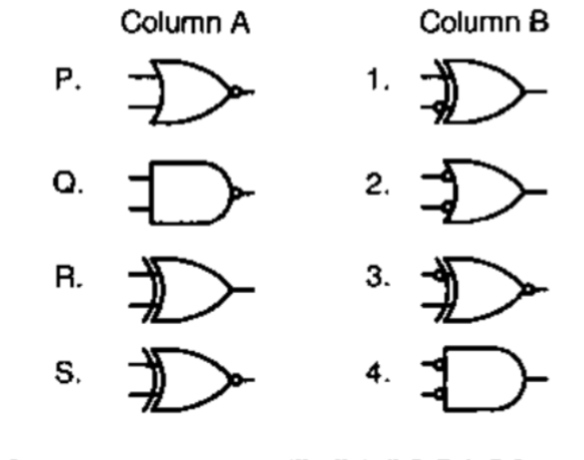
\includegraphics[width=3cm]{GateEC-2010.jpg}
\end{center}

\vspace{0.5cm}

\textbf{Options:}

\begin{enumerate}
\item[(A)] P-2, Q-4, R-1, S-3
\item[(B)] P-4, Q-2, R-1, S-3
\item[(C)] P-2, Q-4, R-3, S-1
\item[(D)] P-4, Q-2, R-3, S-1
\end{enumerate}

\vspace{0.5cm}

\textbf{Solution:}

First identify each gate:

\begin{itemize}
\item \textbf{P:} OR gate with output bubble $\Rightarrow$ NOR gate
\item \textbf{Q:} AND gate with output bubble $\Rightarrow$ NAND gate
\item \textbf{R:} XOR gate
\item \textbf{S:} XOR gate with output bubble $\Rightarrow$ XNOR gate
\end{itemize}

Now identify Column B:

\begin{itemize}
\item \textbf{1:} OR gate
\item \textbf{2:} OR gate
\item \textbf{3:} XOR with output bubble $\Rightarrow$ XNOR
\item \textbf{4:} AND gate
\end{itemize}

\textbf{Matching using logic equivalences:}

\begin{itemize}
\item NOR is equivalent to OR with inverted inputs $\Rightarrow$ matches option 2
\item NAND is equivalent to AND with inverted inputs $\Rightarrow$ matches option 4
\item XOR matches XOR $\Rightarrow$ matches option 1
\item XNOR matches XNOR $\Rightarrow$ matches option 3
\end{itemize}

\[
\boxed{P \rightarrow 2,\quad Q \rightarrow 4,\quad R \rightarrow 1,\quad S \rightarrow 3}
\]

\vspace{0.5cm}

\textbf{Checking Options:}

\begin{itemize}

\item[(A)] P-2, Q-4, R-1, S-3 \\
Correct matching. \textbf{This is the right answer.}

\item[(B)] P-4, Q-2, R-1, S-3 \\
Incorrect: P (NOR) cannot match AND-type gate.

\item[(C)] P-2, Q-4, R-3, S-1 \\
Incorrect: R is XOR but matched with XNOR.

\item[(D)] P-4, Q-2, R-3, S-1 \\
Incorrect: Multiple mismatches.

\end{itemize}

\vspace{0.5cm}

\textbf{Final Answer:} \boxed{(A)}

\end{document}
